\subsubsection{Raspoređivanje kandidata u grupu}
\label{subsubsec:grupe}
\begin{itemize}
  \item \textbf{Kratak opis}: Da bi kandidat bio raspoređen u grupu neophodno je da odabere neku od ponuđenih grupa, nakon logovanja na svoj nalog. 
  \item \textbf{Učesnici}: 
    \begin{itemize}
    \item  Kandidat
    \end{itemize}
  \item \textbf{Preduslovi}:
    \begin{itemize}
    \item Kandidat je dobio svoj ID i lozinku na mejl.
    \end{itemize}
  \item \textbf{Postuslovi}:
      \begin{itemize}
      \item Kandidat je raspoređen u neku grupu.
      \end{itemize}
  \item \textbf{Osnovni tok}:
      \begin{enumerate}
        \item Kandidat se prijavljuje sa svojim ID-jem i šifrom na nalog.
        \item Kandidat klikom na dugme “Grupe” bira neku od ponuđenih grupa.
        \item Sistem šalje mejl kandidatu da je uspešno raspoređen u grupu i raspored održavanja časova.
        \item Kandidat dobija mejl sa podacima o grupi i rasporedu nastave.
      \end{enumerate}

  \item \textbf{Alternativni tokovi}:
      \begin{itemize}
        \item A1. \textbf{Neuspešno prijavljivanje.}
        Kandidat je pogrešio ID ili šifru u koraku 1, pa je nepohodno da proveri ispravnost podataka i da ih ponovo unese. Proces se nastvalja od koraka 1. osnovnog toka.
        \item A2. \textbf{Kandidat nije dobio mejl o raspoređivanju po grupama.}
        Kandidat nije raspoređen u željenu grupu, jer nije dobio mejl sa potvrdom u koraku 4, možda jer je vreme za prijavu isteklo (neko drugi je odabrao preostalo mesto). Proces se nastavlja od koraka 1. osnovnog toka.
      \end{itemize}
\end{itemize}

\begin{figure}[H]
  \begin{center}
      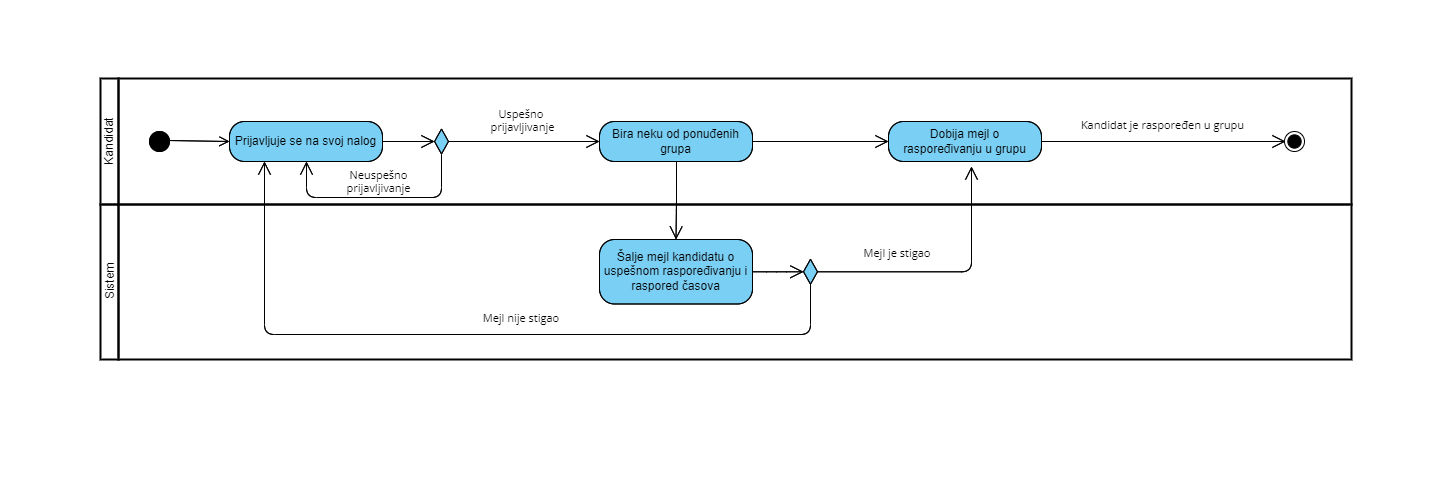
\includegraphics[width=140mm, height=70mm]{Diagrams/dijagram_aktivnosti_grupe.png}
  \end{center}
  \caption {Dijagram aktivnosti - Reaspoređivanje kandidata u grupu}
  \label{activity_grupe}

\end{figure}